\section{Introduction}
\label{sec:introduction}

The rapidly increasing adoption of machine learning (ML) models in a wide range of applications, including healthcare, finance, criminal justice, and autonomous systems, underscores the need for transparency and trust in automated decision-making. However, ensuring the consistency of explanations offered by these models has proven to be a complex challenge with far-reaching implications, particularly in high-stakes scenarios, where decisions carry a substantial impact on individuals and society. This has led to the introduction of various regulatory principles~\citep{aibillofrights, gdpr}.

A key factor complicating the interpretability of predictive models is model indeterminacy, which arises from the existence of multiple (nearly) equally well-performing models for a given dataset and task. Despite comparable performance, these models often provide inconsistent or even contradictory explanations for their decisions (Figure~\ref{fig:toy_example}). Such \textit{explanatory multiplicity} can severely undermine transparency efforts, erode trust in automated decision systems, or lead to potentially harmful outcomes in critical applications such as risk assessment, medical diagnosis, and credit lending.

For instance, in credit lending, a predictive model may be employed to determine a person's creditworthiness. In this context, model indeterminacy can lead to inconsistent explanations for different loan approvals or rejections. An individual might be denied a loan based on one model's decision, while a nearly equally performing model might provide a different explanation and approve the loan. In addition, if a model is periodically retrained without accounting for indeterminacy, it may further exacerbate inconsistencies and erode trust in the decision-making process.\vspace{-1pt}

This prompts us to investigate model indeterminacy in more depth. Specifically, our work examines the \textit{underspecification set} \citep{brunet2022, damour2022} -- the group of models whose performance variations arise solely from changes to the random seed used in training. Similarly performing models from within this set can each offer markedly different explanations for a given input, and prior work has also indicated a notable lack of correlation between the prediction of a model and its explanation \citep{black2021selective, brunet2022}. This raises some important questions. Do equally performing ML models share common patterns in their explanations, or is explanatory multiplicity largely arbitrary? Furthermore, do there exist systematic approaches that can be utilized to align explanations, without compromising on model performance?\vspace{-1pt}

Motivated by these questions, we propose the use of ensemble methods to mitigate explanatory multiplicity among equally performing neural networks (Figure~\ref{fig:toy_example}), and explore the application of various ensemble methods towards improving the consistency of explanations generated for this class of models. Focusing on neural networks is particularly relevant to this problem setup, given their expressivity and ability to fit complex functions. Neural networks of sufficient size can cover a large range of predictors, even for relatively small tasks. Our aim is to devise efficient ensembling strategies that can align explanations across various diverse modes, while simultaneously requiring fewer pre-trained models to do so. The methods deployed are informed by previous research on neural network loss landscapes and existing explanation techniques.\vspace{-1pt}

More specifically, our overall contributions are as follows:\vspace{-1pt}

\begin{enumerate}
    \item In \S\ref{sec:ensembles}, we propose ensemble strategies that target two facets of the neural network loss landscape: local perturbations on model weights (\S\ref{subsec:ensembles_weight}); and global connections between models along paths of near-constant loss (\S\ref{subsec:ensembles_mode}). We provide a toy illustration to demonstrate how explanatory multiplicity can be mitigated through both types of exploration (\S\ref{subsec:ensembles_illustration}).
    \item In \S\ref{subsec:experiments_weight}, we perform ablations to understand the impact of weight perturbations on explanation similarity, finding that it depends critically on the layer being perturbed. %In \S\ref{subsec:experiments_mode}, we analyze the paths that connect models globally, finding that they are often 
    \item In \S\ref{subsec:experiments_ensemble}, we conduct experiments across five benchmark financial datasets and three commonly used explanation techniques, demonstrating that ensembles constructed through local or global exploration of the loss landscape can yield significant improvements in terms of average pairwise top-$k$\footnote{For a given explanation, the $k$ largest features according to absolute value.} similarity between explanations. We further showcase how a novel combination of both local and global ensembling can yield performance improvements up to fivefold over naive ensembling, given a fixed number of pre-trained models.%
\end{enumerate}\vspace{-1pt}
%\suraj{contributions list should be specific and concrete with respect to what is done various sections of the paper - we propose this, we experimentally find that, we prove this, etc }

\begin{figure}[t]
    \centering
    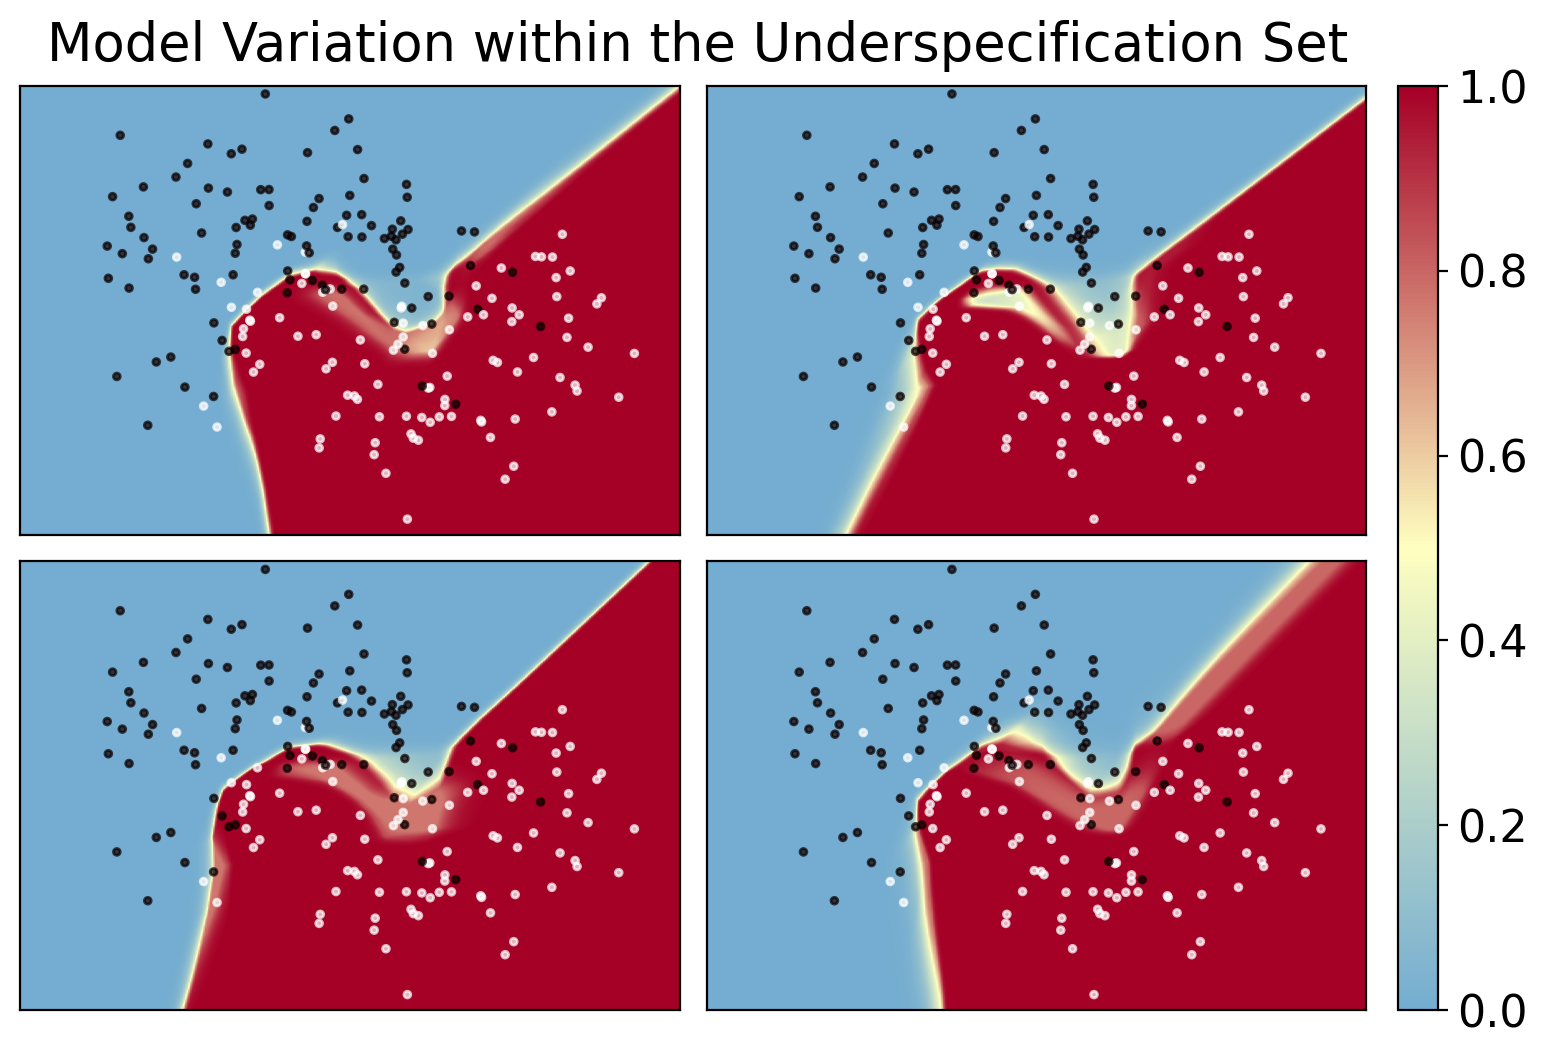
\includegraphics[width=0.3135\textwidth]{figures/toy_underspec.png}
    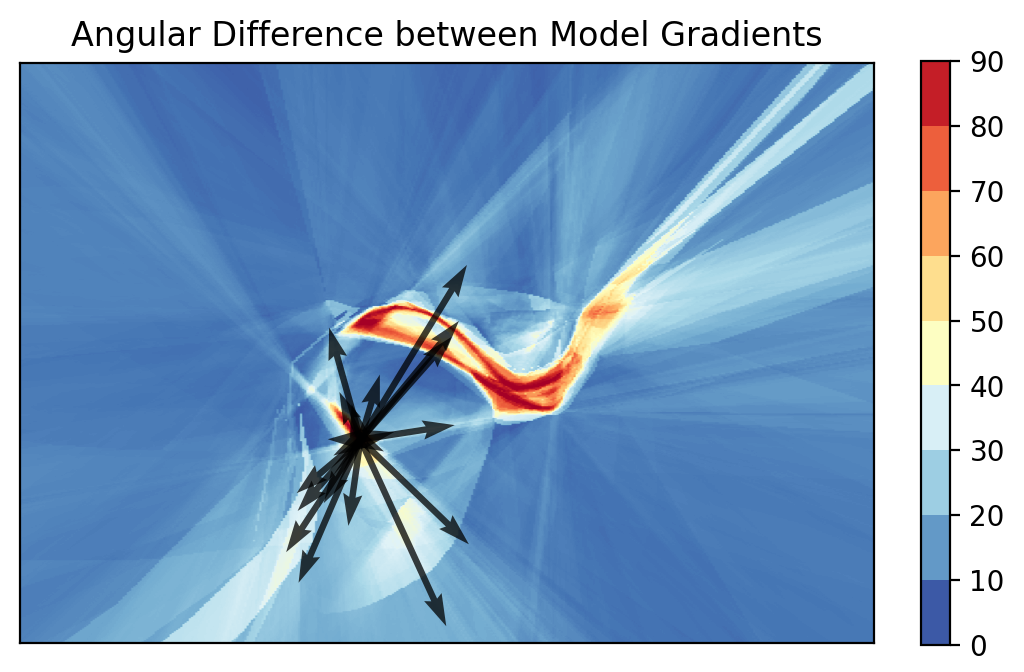
\includegraphics[width=0.33\textwidth]{figures/toy_single.png}
    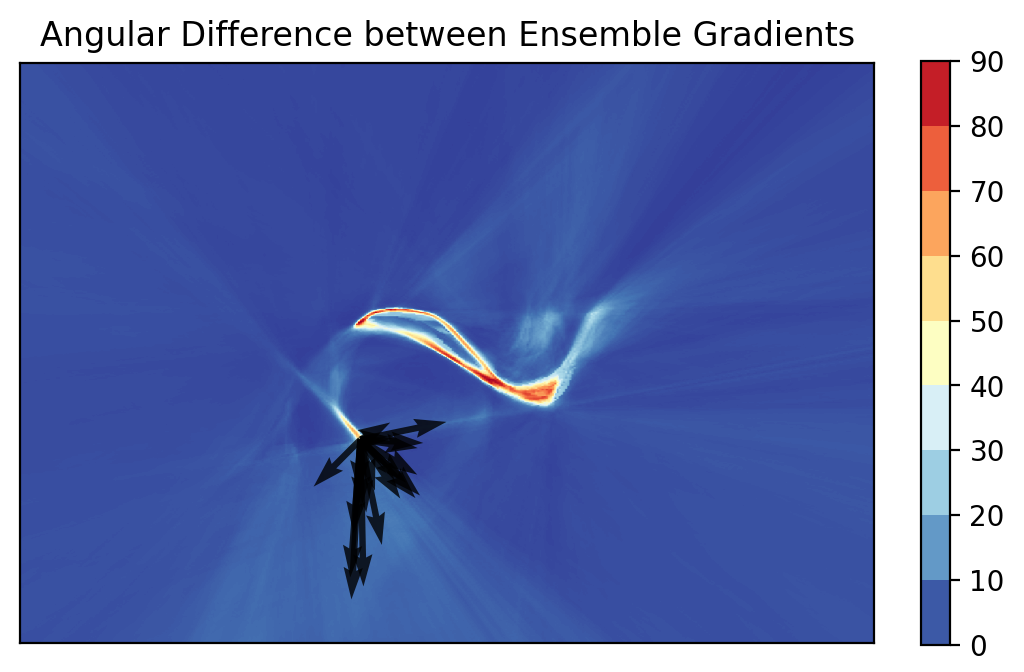
\includegraphics[width=0.33\textwidth]{figures/toy_ensemble.png}
    \caption{\small Illustration of explanatory multiplicity between members of the underspecification set (model variation due only to random seed). \textbf{Left:} softmax probabilities of neural networks trained on the two moons dataset, with test points depicted in black and white. All models achieve similar performance on test data. \textbf{Center:} average pairwise angular difference between model explanations in the same region of input space. Gradients with respect to the input, a proxy for many explanation techniques, are shown for a test point of high disagreement (i.e. high angular difference) between models. \textbf{Right:} average pairwise angular difference between ensemble explanations. Ensembles consist of 10 constituent models sampled from the underspecification set. Our findings indicate that \textit{ensembling results in model alignment, promoting agreement between explanations in input space.}}
    \label{fig:toy_example}
\end{figure}%\vspace{-5pt}

While our experiments highlight the potential of ensemble techniques in alleviating the challenges posed by model indeterminacy, the problem of providing consistent explanations for ML models remains an ongoing area of research. This work seeks to contribute to the development of more  trustworthy and reliable ML systems that can be implemented responsibly in high-stakes, real-world applications, and provides an empirical analysis of ensemble behavior in such regards.

%\paragraph{Include references:} \citet{aibillofrights, gdpr}
